\documentclass[12pt]{article}
\usepackage[english]{babel}
\usepackage{natbib}
\usepackage{url}
\usepackage[utf8x]{inputenc}
\usepackage{amsmath}
\usepackage{graphicx}
\graphicspath{{images/}}
\usepackage{parskip}
\usepackage{fancyhdr}
\usepackage{vmargin}
\usepackage{float}
\usepackage{hyperref}
\setmarginsrb{3 cm}{2.5 cm}{3 cm}{2.5 cm}{1 cm}{1.5 cm}{1 cm}{1.5 cm}

\title{Finite Element Based Structural Analysis Software}								% Title
\author{Group 20}								% Author
\date{20 Jan 2019}											% Date

\makeatletter
\let\thetitle\@title
\let\theauthor\@author
\let\thedate\@date
\makeatother

\pagestyle{fancy}
\fancyhf{}
\rhead{\theauthor}
\lhead{\thetitle}
\cfoot{\thepage}

\begin{document}

%%%%%%%%%%%%%%%%%%%%%%%%%%%%%%%%%%%%%%%%%%%%%%%%%%%%%%%%%%%%%%%%%%%%%%%%%%%%%%%%%%%%%%%%%

\begin{titlepage}
	\centering
  %  \vspace*{0.5 cm}
    
\includegraphics[scale = 0.75]{logo.jpg}\\[1.0 cm]	% University Logo
    \textsc{\LARGE Department of Computer Engineering \newline\newline University of Peradeniya}\\[1.0 cm]	% University Name
	\textsc{\Large CO328 Software Engineering Project}\\[0.5 cm]				% Course Code
	\rule{\linewidth}{0.2 mm} \\[0.4 cm]
	{ \huge \bfseries \thetitle}\\
	\rule{\linewidth}{0.2 mm} \\[0.5 cm]
	
	\begin{minipage}{0.8\textwidth}
		\large \emph{Group 20:}\\
			\begin{tabular}{l l}
			     E/14/158&Gihan Jayatilaka\\
			     E/14/339&Suren Sritaharan\\
			     E/14/379&Harshana Weligampola\\
			\end{tabular}
			\vspace{1cm}
			
		\large \emph{Client:}\\
		     Structures Laboratory,\\ Department of Civil Engineering,\\ University of Peradeniya.\\
	
			\end{minipage}~
			\begin{minipage}{0.8\textwidth}
            

        
	\end{minipage}\\
	
	
    
    
    
    
	
\end{titlepage}

%%%%%%%%%%%%%%%%%%%%%%%%%%%%%%%%%%%%%%%%%%%%%%%%%%%%%%%%%%%%%%%%%%%%%%%%%%%%%%%%%%%%%%%%%

\tableofcontents
\pagebreak

%%%%%%%%%%%%%%%%%%%%%%%%%%%%%%%%%%%%%%%%%%%%%%%%%%%%%%%%%%%%%%%%%%%%%%%%%%%%%%%%%%%%%%%%%

\section{Abstract}
Finite Element Method (FEM) is widely used for structural analysis in civil engineering projects. FEM algorithms predict the deformations and failures of structures under different loading conditions. These algorithms are computationally intensive.\\
The most popular method to perform nonlinear analysis is force based fiber beam column element. A newer (and better) formulation has been proposed by University of Peradeniya\cite{chathura-paper}. This algorithm has been experimentally proven to be giving stable and accurate solutions with respect to axial force - bending moment interaction of civil engineering structures.\\
A computationally efficient implementation of this algorithm with a user friendly interface is crucial in making this theoretical advance usable for practical applications.\\ 
This CO328 project tries to implement a usable version of the proposed algorithm and test it against manually calculated structural deformation predictions. The software program will be packaged in a way that it can act as the backend for the "CO328 project - Structural Analysis Project". Furthermore, the software will contain an API to enable it to be used as the building block of algorithms built on this proposed formulation.\\
\section{Introduction}

\section{Related work}

\subsection{Related algorithms}

\subsubsection{Classical methods}
These algorithms are usually studied in the first part of the undergraduate curriculum. They can solve simple structures. But they fail to analyze complicated structures.\\ Method of joints and method of sections cannot be used to analyze the deformations (linear elastic and plastic) or the failure for the structure since they work on the assumption that all elements of the structure are ideal. Elasticity based methods can analyze linear elastic deformations only.\\
\begin{itemize}
    \item Method of joints\\
    \begin{figure}[H]
        \centering
        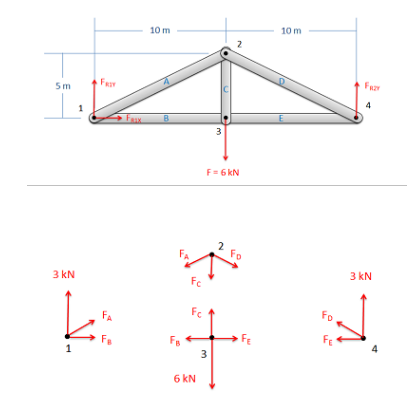
\includegraphics{images/methodOfJoints.png}
        \caption{Method of joints}
        \label{fig:jointsMethod}
    \end{figure}
    The method of joints is a process used to solve for the unknown forces acting on members of a truss. The method centers on the joints or connection points between the members, and it is usually the fastest and easiest way to solve for all the unknown forces in a truss structure.\cite{adaptive-map}


    \item Method of sections\\
    \begin{figure}[H]
        \centering
        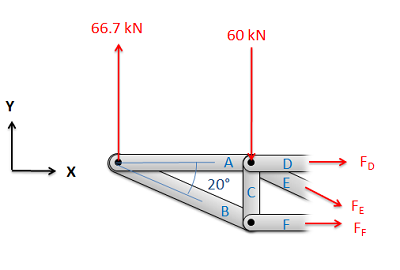
\includegraphics{images/sectionsMethod.png}
        \caption{Method of sections}
        \label{fig:sectionsMethod}
    \end{figure}
    The method of sections is a process used to solve for the unknown forces acting on members of a truss. The method involves breaking the truss down into individual sections and analyzing each section as a separate rigid body. The method of sections is usually the fastest and easiest way to determine the unknown forces acting in a specific member of the truss.\cite{adaptive-map}
    \item Elasticity based methods\\
    Elasticity methods are available generally for an elastic solid of any shape. Individual members such as beams, columns, shafts, plates and shells may be modeled. The solutions are derived from the equations of linear elasticity. The equations of elasticity are a system of 15 partial differential equations. Due to the nature of the mathematics involved, analytical solutions may only be produced for relatively simple geometries.\cite{wiki-structures}
    
\end{itemize}
% @GIHAN

\subsubsection{Numerical methods}
It is common practice to use approximate solutions of differential equations as the basis for structural analysis. This is usually done using numerical approximation techniques.
\begin{itemize}
    \item Finite difference methods
    \item Finite element methods
\end{itemize}
% @GIIHAN RESIZE

\subsection{Related software packages}
\subsubsection{SAP 2000}
\begin{figure}
    \centering
    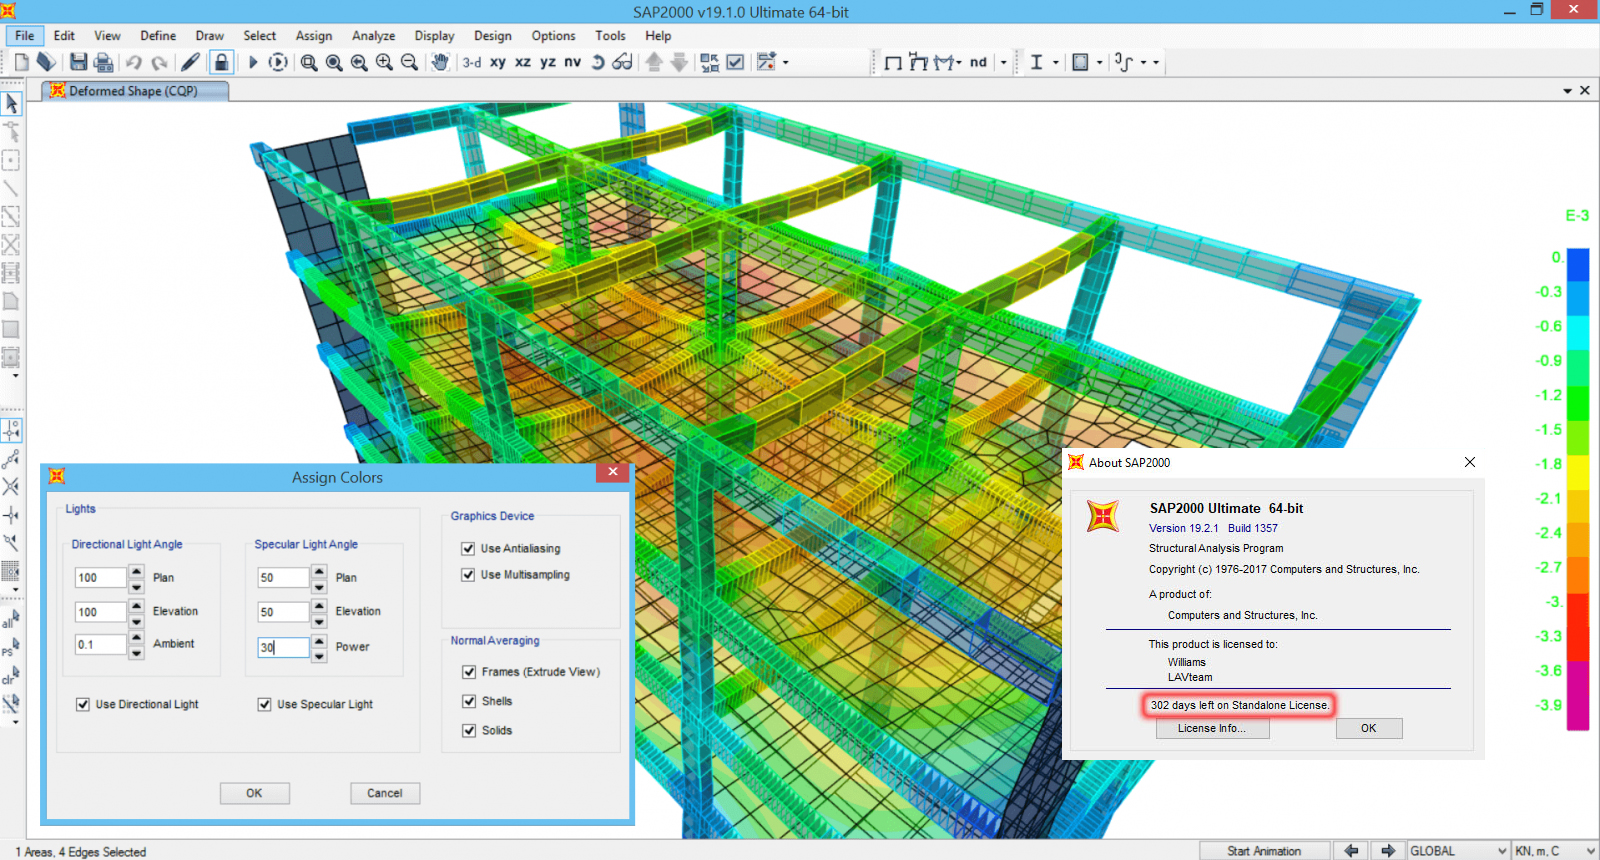
\includegraphics[scale=0.2]{images/sap.jpg}
    \caption{SAP2000 Structural Analysis Software}
    \label{fig:my_label}
\end{figure}
SAP2000 is the industry standard structural analysis software. It has been used on every form of structural design ranging from simple structures for Burj Khalifa.\\

\textbf{Pros:} Industry standard\\
\textbf{Cons:} This does not allow non-linear analysis.\\
\subsubsection{S-FRAME Analysis}
\begin{figure}[H]
    \centering
    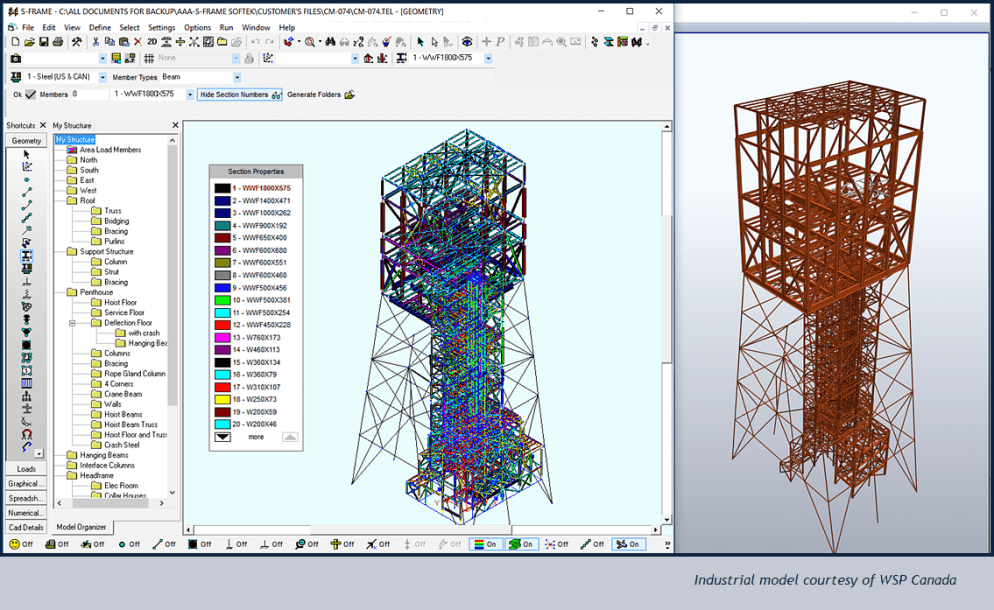
\includegraphics[scale=0.3]{images/sFrame.png}
    \caption{S-FRAME Structural Analysis Software}
    \label{fig:my_label}
\end{figure}
\textbf{Pros:} Can perform non linear analysis.\\
\textbf{Limitations:} \begin{itemize}
    \item Cannot analyze the bending moment, axial force interaction.
    \item Expensive
\end{itemize}
% @GIIHAN RESIZE



\section{Proposed Solution}
\subsection{Introduction}
The project aims to create a software capable of running a structural analysis on a given civil engineering structure. The program will be able to asses the response of the structure against different loading conditions.\\
The software will use industry standards from SAP2000 for structural element definitions and coordinate systems.\cite{sap-ref} 

\subsection{Formulation}
\subsubsection{Coordinate system}
The global coordinate system is a three-dimensional, right-handed, rectangular coordinate system. The three axes, denoted X, Y, and Z, are mutually perpendicular and satisfy the right-hand rule. The location and orientation of the global system are arbitrary.\\ Locations in the global coordinate system can be specified using the variables x, y, and z. A vector in the global coordinate system can be specified by giving the locations of two points, a pair of angles, or by specifying a coordinate direction. Coordinate directions are indicated using the values ±X, ±Y, and ±Z. For example, +X defines a vector parallel to and directed along the positive X axis. The sign is required. \\ All other coordinate systems in the model are defined with respect to the global coordinate system.

\subsubsection{Frame element}
The Frame element uses a general, three-dimensional, beam-column formulation which includes the effects of biaxial bending, torsion, axial deformation, and biaxial shear deformations. See Bathe and Wilson (1976).\\
Structures that can be modeled with this element include:
\begin{itemize}
    \item Three-dimensional frames
    \item Three-dimensional trusses
    \item Planar frames
    \item Planar grillages
    \item Planar trusses
\end{itemize}
A Frame element is modeled as a straight line connecting two joints. Each element has its own local coordinate system for defining section properties and loads, and for interpreting output.\\
Each Frame element may be loaded by self-weight, multiple concentrated loads and multiple distributed loads.

\subsubsection{Connectivity}
Every frame element is connected at two end nodes. It may be connected to one or more elements at those ends.
\subsubsection{Degrees of freedom}
Every frame element has 6 degrees of freedom.

\subsection{Algorithm}
The algorithm consists of the following steps.\\
\begin{enumerate}
    \item \textbf{Take inputs}\\
    The inputs are read from the standard format file. 
    \item \textbf{Create local stiffness matrices}\\
    The stiffness matrices for every element is created using it's properties (length, cross section area, young's modulus). The coordinate system at this stage is the local coordinate system.\\
    Given that the degrees of freedom per node is 6 and an element has 2 degrees of freedom $$K_{local 12\times12}$$
    \item \textbf{Global stiffness matrix}\\ The global stiffness matrix is the characteristic function defining the load response of a structure. This is a square matrix of $no\_of\_nodes \times dof\_per\_node$. There are two steps required to generate this matrix.
    \begin{itemize}
        \item Rotate the local stiffness matrices (according to the orientation of the element)
        \item Add the resultant element stiffness matrix elements to the relevant elements in the global stiffness matrix.
    \end{itemize}
    
    $$K_{global (N \times N)}$$
    
    \item \textbf{Generate the external load matrix}\\
    This is done by placing the external torques and forces in a column matrix.
    $$F_{(N \times 1)}$$
    \item \textbf{Handle fixed points}\\
    It is already known that the deformation at fixed points should be zero. Therefor all the row and column vectors corresponding to the fixed points in the global stiffness matrix are removed to obtain the reduced stiffness matrix.
    
    \item \textbf{Solving}\\
    Now a linear system $F = K_{red}X$ is obtained where $F$ is the load vector, $K_{red}$ is the reduced global stiffness matrix and $X$ is the deformation vector. The system should be solved for $X$ as $$X = F^{-1}K_{red}$$ This is the most computationally heavy operation of the program.
    
    \item \textbf{Backtracking the deformation} \\
    The solution obtained up to now is for the displacement of nodes in global coordinate system. This is backtracked to the displacement of nodes in the local coordinate systems of elements. That can be traced back to the deformation and the forces acting on the elements.
    
    \item \textbf{Output}
    The output is genearated in a standard format for the GUI program. It is algo dumped to a file on disk.\\
\end{enumerate}

\subsection{Software}
The software product of the project is a easy to use shell application that can perform the above mentioned structural analysis. The core functionality will be released on two forms.
\begin{itemize}
    \item A standalone application that can perform the analysis
    \item A python package that can be integrated into GUI software (Group 17) or other complex software taking use of this analysis technique.
\end{itemize}
\section{Implementation}
% @HARSHANA
Since the algorithm executes in the back-end, it should be written in an efficient and reliable language. The I/O of the back-end was handled by Python. Then, the algorithm was developed in 3 parallel branches that used python, cuda and MATlab as the programming language. The MATlab and python solutions were released early because they can be implemented fast. Cuda implementation was developed to a similar stage but further development came to a halt due to customer requirement to implement the algorithms using solely on python.

\subsection{Design}
The complexity lies in the algorithms and the data structures. Thus, the design of the software is simple. The software works as an interface for the front end. So the requirements are well defined and constrained.

In the context of this software, elements are the major classes of each structure. Almost all the elements have similar properties, thus they inherit their attributes from a generic element. The elements differ only in certain attributes known as the "degree of freedom" which varies between each element.

% @GIHAN @Harshana insert design diagram
\subsection{Technology stack}

% @HARSHANA
The software is made using python. The algorithmic implementation was also made in C++, cuda and MATLAB but due to the limited requirement of the project owner, these versions were not released (The development version of these implementations can be found in the development branch of the github repository).

% @GIIHAN @HARSHANA
The following packages were used:
\begin{itemize}
    \item json: Read and write json files which is the agreed format of communication with the front end.
    \item numpy : Used for mathematical computation
    \item scipy : Used for efficient linear solving
    \item unittest : Used for testing
    \item cuBLAS : Used for basic linear algebraic operations
\end{itemize}


\section{Agile development practices}

A major reason for the success of this project was due to the agile development practices which were followed. These practices ensured a smooth development process. Few of the agile development practices which were followed have been explained in detail below.

\subsection{Collaboration}
The project was done in collaboration with 2 other groups with the final objective of integrating the work of all 3 groups to form a fully working product. The work was divided between the three teams considering the specialization of each groups. As such, the task which was handed over to us was the formulation, design and optimization of the Finite Element based algorithm for Structural analysis.

\begin{figure}[H]
    \centering
    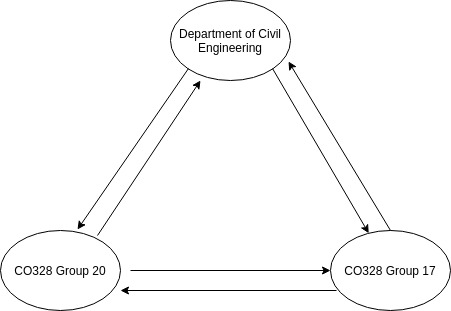
\includegraphics[scale=0.5]{images/GroupInteractions.jpeg}
    \caption{Group interactions}
    \label{fig:groups}
\end{figure}

\begin{figure}
    \centering
    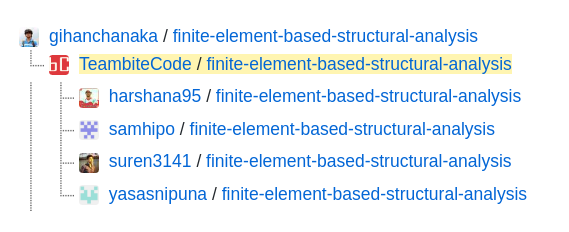
\includegraphics[scale=0.5]{images/github.png}
    \caption{Github repo with both Group 20 and the Client}
    \label{fig:my_label}
\end{figure}



\begin{tabular}{|l| l|}
    \hline
    Stakeholder & Description\\
    \hline
     Department of Civil Engineering & Client \\
     Group 17 & GUI development\\
     \textbf{Group 20} & \textbf{Backend developemnt}\\
     \hline
\end{tabular}

\subsubsection{Collaboration within Group 20}

\begin{itemize}
    \item Informal scrum meetings to plan, discuss.
    \item An email thread to set goals.
    \item Github to share code and collaborate work.
\end{itemize}
% @HARSHANA insert pic here of github contrib
\begin{figure}[H]
    \centering
    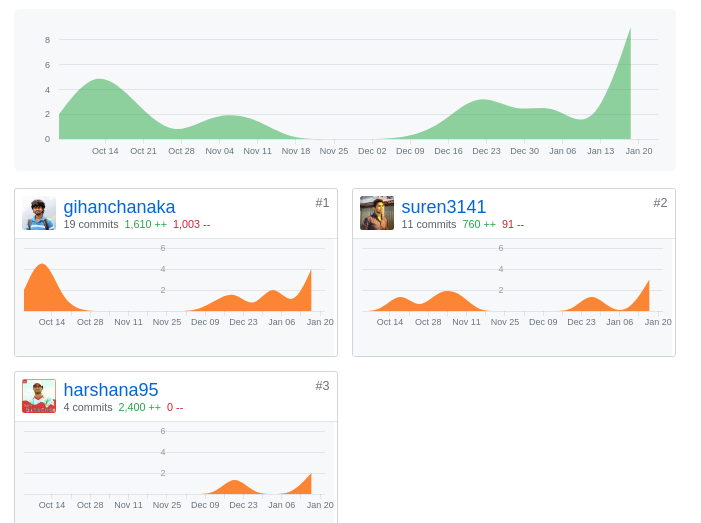
\includegraphics[scale=0.5]{images/git-contrib.png}
    \caption{Contribution graph}
    \label{fig:my_label}
\end{figure}

\subsubsection{Collaboration of Group 20 with Civil Engineering Department}

\begin{itemize}
    \item Weekly meetings (for first few weeks) for domain familiarization.
    \item Bi-weekly meetings (after first few weeks) to discuss the progress, clear doubts.
    \item Email thread
\end{itemize}

\subsubsection{Collaboration of Group 20 with Group 17}

A common interface (data saving format) had to be agreed upon for both groups to start work. This was critical for the project since every next step is dependent on this. The discussions were done in meetings but the final decisions were always sent via email. The sample data saving formats were shared through github.\\

\begin{itemize}
    \item Email thread to communicate the interface
    \item Github For code sharing
\end{itemize}

\subsubsection{Collaboration of Group 17 with the Civil Engineering Department}
This is out of the scope of this report.\\


\subsection{Test driven development}
Automated test cases play an important role in agile development. Constructing test cases together with the requirement engineering process not only ensures that the groups have significant clarity on their requirements; but it also helps to continuously test the code throughout the developments process. As such, tests were made based on 2 criteria:
\begin{itemize}
    \item Use case testing
    \item Performance Testing
\end{itemize}


\subsubsection{Use case testing}
Use case test were constructed to ensure that the software satisfied the functional requirements of the user. In the context of this project the test cases which were generated at the beginning was the physical structures and their corresponding analytically values. These were used for integration / black box tests at the end of the project.\\
Apart from these, before the beginning of each task, specific test cases were created to ensure that each section of the code functioned properly. These acted as unit tests.\\
Python unittest module was used to test the code. Integration tests were done before each releases, but unit tests were done after each update / re-factoring.\\

\begin{figure}[H]
    \centering
    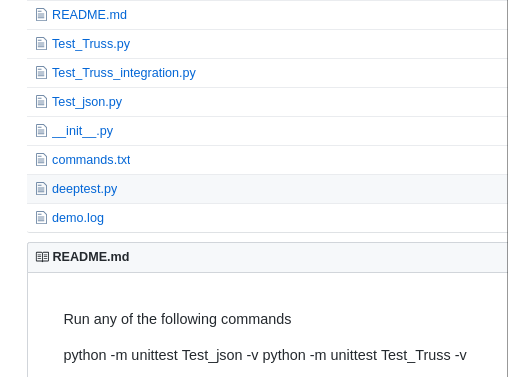
\includegraphics[scale=0.4]{images/tests.png}
    \caption{Use case testing scripts}
    \label{fig:my_label}
\end{figure}

\subsubsection{Performance testing}

This software is a CPU heavy computation. It is crucial to test it for performance to ensure that it will be usable for the internded purposes.\\Usually the civil engineering structures have a large number of elements. The polynomial time algorithm may take longer time periods to give results. Therefor, the software was tested with different algorithms to make sure that it performs the computation in a time period which is not more than what the existing industrial solutions need.\\ 

\begin{figure}[H]
    \centering
    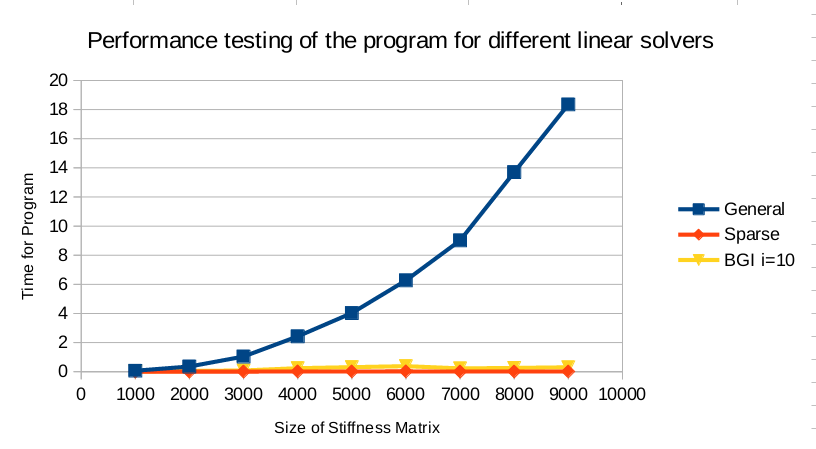
\includegraphics[scale=0.5]{images/performance}
    \caption{Performance testing}
    \label{fig:my_label}
\end{figure}


\subsection{Continuous integration}
Agile development places significant importance on working software and it's codes over planning and documentation: The argument being that a working software could be easily evaluated by the customers and other team members as opposed to an abstract design.

%% @ HARSHANA
% @GIIHAN do we mention versions, branches
To facilitate continuous development and integration github was used as the online platform for collaborative coding. The figure shows the contributions of each member of the group.\\


\begin{figure}[H]
    \centering
    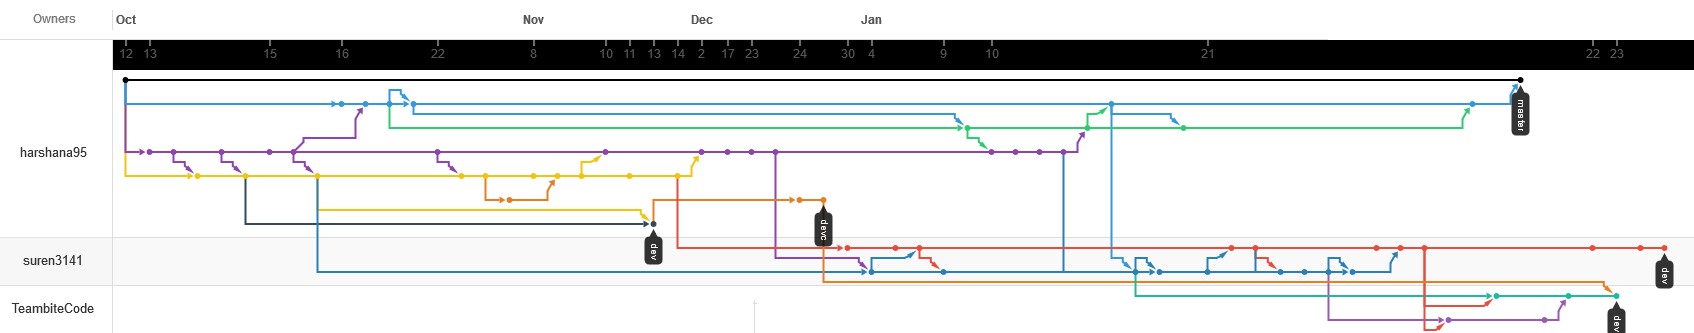
\includegraphics[width=\textwidth]{images/canvas.png}
    \caption{Network of contributions}
    \label{fig:groups}
\end{figure}

\subsubsection{Branches}
In order to have a clear understanding the repository was divided into 2 branches: development and master. \\

\textbf{Dev branch: } All the group members push to their dev branch. They may pull from any other member's dev branch. Finally, once a milestone is reached, a member sends a pull request to the Team dev branch. After discussion, the scrum master pulls to the team dev branch.\\

\textbf{Master branch: } Individual group members do not push to their own master branch. The team discusses and pushes to the team's master branch from it's dev branch. The individual members may pull from the team maaster branch.\\
Master branch is also used as a reference for other group members (Civil Engineering Department and Group 17.\\



\subsection{Timeline}
% @GIIHAN @HARSHANA
The time line agreed with the project owner is shown below.\\
\begin{figure}[H]
    \centering
    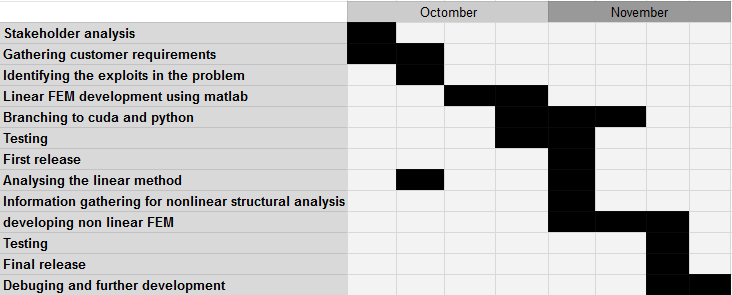
\includegraphics[width=\textwidth]{images/timeline.png}
    \caption{Planned time-line for the project}
    \label{fig:groups}
\end{figure}

As shown, the project is expected to be completed by the end of the year. Within the current academic semester only part of it was expected to be completed. As per this requirement, the linear solver has been developed and the interface has been completed for deployment .Therefore, for the CO328 : Software engineering course only this section has been completed and presented.\\
Additionally, the non-linear solvers have been developed, but requires testing to ensure that it works according to the customer requirements.

\subsection{Releases}

The software is released by the name \textbf{fem-struct} (Finite Element Method based STRUCTURAL analysis software). There are two versions given for different use cases.\\


\begin{itemize}
    \item \textbf{Standalone software}\\
    This is released on github releases.\\
    \href{https://github.com/TeambiteCode/finite-element-based-structural-analysis/releases}{https://github.com/TeambiteCode/finite-element-based-structural-analysis/releases}\\
    This can be installed by running the script \textbf{install.sh}
    Then the program can be called by the shell keyword \textbf{fem-struct}.
    \item \textbf{Python package}\\
    \href{https://test.pypi.org/project/fem-struct/}{https://test.pypi.org/project/fem-struct/}\\
    This can be installed by the command\\
    \textbf{pip install -i https://test.pypi.org/simple/fem-struct}\\
    
    
    
    
\end{itemize}

\section{Conclusion}
%@GIHAN
The major objective of this software was to optimize the algorithm as well as  it's implementation to achieve better performance considering both the time as well as the memory. Algorithmic optimization was the priority requirement of the project owner, and the given implementation was able to provide a 100x speedup.
Although code optimization was a minor concern a significant improvement was achieved using good coding practices and re-factoring.\\

The entire algorithm is expected to be completed by the end of the year and would be integrated with the components made by the two other groups (front-end, manuals, etc) to form the final product.

\section{Future work}
The software developed until now concentrates only on linear solvers. Since there are many other alternative software which provide similar performances, the major part of the software would be the non-linear solver.\\

Although significant speedup was achieved through the modified implementation, the efficiency could be further improved. Especially parallel and low level (assembly) implementations could be considered as alternatives for this issue. Furthermore other techniques which could exploit the structure of the matrices (sparsity) were not analyzed in detail when improving the time efficiency of the algorithm. Having a deeper understanding of this structure could be vital in improving the efficiency.\\





\newpage
\bibliographystyle{plain}
\bibliography{biblist}

\end{document}